\documentclass[12pt,letterpaper]{article}

\usepackage[utf8]{inputenc}
\usepackage[letterpaper,margin=1in]{geometry}
\usepackage{caption} % for table captions

\usepackage{amsmath} % for multi-line equations and piecewises
\usepackage{indentfirst} % to indent after a section
\usepackage{setspace}
\usepackage{times}
\usepackage{graphicx}
\usepackage{textcomp}
\usepackage{xspace}
\usepackage{verbatim} % for block comments
\usepackage{subfig} % for subfigures
\usepackage{enumitem} % for a) b) c) lists
\usepackage{float}
\newcommand{\Cyclus}{\textsc{Cyclus}\xspace}%
\newcommand{\Cycamore}{\textsc{Cycamore}\xspace}%
\usepackage{titling}
\usepackage{listings}
\newcommand{\subtitle}[1]{%
  \posttitle{%
    \par\end{center}
    \begin{center}\large#1\end{center}
    \vskip0.5em}%
}
\usepackage{tikz}

\definecolor{listinggray}{gray}{0.9}
\definecolor{lbcolor}{rgb}{186,255,241}
\definecolor{antiquefuchsia}{rgb}{0.57, 0.36, 0.51}
\definecolor{aquamarine}{rgb}{0.5, 1.0, 0.83}
\definecolor{prettygreen}{rgb}{153,255,51}
\lstset{
    backgroundcolor=\color{prettygreen},
    tabsize=4,
  language=C++,
  captionpos=b,
  tabsize=4,
  frame=lines,
  numbers=left,
  numberstyle=\tiny,
  numbersep=5pt,
  breaklines=true,
  showstringspaces=false,
  basicstyle=\footnotesize,
  }


\lstdefinelanguage{XML}
{
  morestring=[b]",
  morestring=[s]{>}{<},
  morecomment=[s]{<?}{?>},
  stringstyle=\color{black},
  identifierstyle=\color{red},
  keywordstyle=\color{cyan},
  morekeywords={xmlns,version,type}% list your attributes here
}

\usetikzlibrary{shapes.geometric,arrows}
\tikzstyle{process} = [rectangle, rounded corners, minimum width=3cm, minimum height=1cm,text centered, draw=black, fill=blue!30]
\tikzstyle{arrow} = [thick,->,>=stealth]


\graphicspath{{images/}}
 
\usepackage[font={footnotesize,it}]{caption}
 



\setlength{\parindent}{15pt} % Default is 15pt.




\fontfamily{ptm}\selectfont

\title{Numerical Experiments for Verifying Demand Driven Deployment Algorithms}
\subtitle{Draft 1}
\author{Jin Whan Bae and Gwendolyn Chee}
\date{2017-09-23}


\begin{document}
	
	\maketitle
	\hrule
	\onehalfspacing
	\thispagestyle{empty}

\section*{Introduction}
The Demand-Driven Cycamore Archetype project (NEUP-FY16-10512) aims to develop \Cycamore demand-driven deployment capabilities.
The project plans to use non-optimizing, deterministic-optimizing and stochastic-optimizing prediction algorithms.

These prediction models are being developed by the University of South Carolina. In this report, we discuss numerical experiments for testing the non-optimizing, deterministic optimizing and stochastic optimizing methods. 

\section{Once through Nuclear Fuel Cycle}
This section defines the required tests for
each method assuming a once-through fuel cycle.

\begin{figure}[H]
\caption{Flow Chart of Once through Nuclear Fuel Cycle}
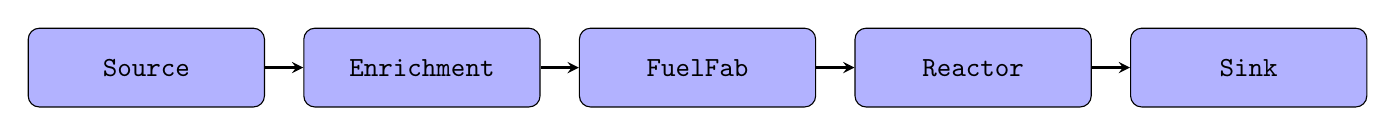
\begin{tikzpicture}[node distance=3.5cm]
\node (source) [process] {\texttt{Source}};
\node (enrichment) [process, right of=source] {\texttt{Enrichment}};
\node (fuelfab) [process, right of=enrichment] {\texttt{FuelFab}};
\node (reactor) [process, right of=fuelfab]{\texttt{Reactor}};
\node (sink) [process, right of=reactor]{\texttt{Sink}};

\draw [arrow] (source) -- (enrichment); 
\draw [arrow] (enrichment) -- (fuelfab); 
\draw [arrow] (fuelfab) -- (reactor);
\draw [arrow] (reactor) -- (sink);
\end{tikzpicture}
\end{figure}

\section{Input File Specification}
We assume the archetype to be an \texttt{INSTITUTION}, since
it governs deployment and decommission of facilities.

The user would only have to define the reactor prototype and reactor deployment. 
The remaining fuel facilities,
both front end and back end, would be recognized by the archetype
by looking at each prototypes' in-and-out commodities.
Then the recognized, or `connected' fuel cycle facilities deploy
with demand.
If an input file does not have the necessary `connections' for the 
reactor to receive fuel, it will throw an error. 

We suggest an example format:
First, the input file would define reactor prototype to be deployed. There can be multiple reactors.
\begin{lstlisting}[language=XML, caption=One-reactor fleet institution input schema]
<institution>
      <name>NO_ddd</name>
       <config><NO_ddd/></config>
      <reactor_list>
        <val>lwr</val>
        <val>sfr</val>
        <val>mox_lwr</val>
      </reactor_list>
\end{lstlisting}

[Something About Transition Scenario Capabilities]

Then deployment of the reactors is defined, and the user
is given the option to manually define the deployment(DeployInst):
\begin{lstlisting}[language=XML, caption=Reactor deployment input schema]
      <deployment>
      <type>manual</type>

        <build_times>
          <val>1</val>
          <val>10</val>
          <val>20</val>
          <val>40</val>
        </build_times>
        <n_build>
          <val>3</val>
          <val>3</val>
          <val>3</val>
          <val>3</val>
        </n_build>
        <lifetimes>
          <val>960</val>
          <val>960</val>
          <val>960</val>
          <val>960</val>
        </lifetimes>
      </deployment>

    </institution>
\end{lstlisting}

or have the institution
deploy reactors according to power demand (GrowthRegion):

\begin{lstlisting}[language=XML, caption=Reactor deployment input schema]
      <deployment>
      <type>growth</type>

      <growth>
        <piecewise_function>
              <piece>
                <start>0</start>
                <function>
                  <type>linear</type>
                  <params>1 2</params>
                </function>
              </piece>
        </piecewise_function>
      </growth>
      
      </deployment>

    </institution>
\end{lstlisting}

\subsection{Non-optimizing prediction method}
The following conditions need to be satisfied.

\begin{enumerate}
\item  Do all the \texttt{Reactor}s run at full capacity (not lacking fuel)? 

\item Is the predicted fuel demand within a specific uncertainty of the analytic solution? 

\item  Is the output of the \texttt{Fuelfab} within a specific range (more than?) of the input required by the \texttt{Reactor}s (calculated by the analytic solution) for all of them to run for each time step? 
\begin{itemize}
\item Is a new \texttt{Fuelfab} deployed when the input required by the reactors exceeds the output of current \texttt{Fuelfab}?

\item Is a \texttt{Fuelfab} decommissioned when the input required by the reactors falls behind the output of current \texttt{Fuelfab} facilities?
\end{itemize}

\item  Is the output of the \texttt{Enrichment} within a specific range of the input required by the \texttt{Fuelfab} (calculated by the analytic solution) for each time step? 
\begin{itemize}
\item Is a new \texttt{Enrichment} deployed when the input required by the \texttt{Fuelfab} exceeds the output of current \texttt{Enrichment} facilities?
\item Is a \texttt{Enrichment} decommissioned when the input required by the \texttt{Fuelfab} falls behind the output of current \texttt{Enrichment}?
\end{itemize}

\item Is the output of \texttt{Source} within a specific range of the input required by the \texttt{Enrichment} (calculated by the analytic solution) for each time step? 
\begin{itemize}
\item Does the \texttt{Source} output increase when the input required by the \texttt{Enrichment} exceeds the output of current \texttt{Source}?
\item Does the \texttt{Source} output decrease when the input required by the \texttt{Enrichment} falls behind the output of current \texttt{Source}?
\end{itemize}


\end{enumerate}


However, the user may not have his or her cycle set to the generic fuel cycle, and may have
variations so that there is no \texttt{Fuelfab} or \texttt{Enrichment}, but the fuel is
directly supplied by the \texttt{Source}. This brings the need for the algorithm to recognize
the supply chain the supply fuel to the reactor, and deploy necessary facilities accordingly. 


\subsection{Deterministic-Optimizing/Stochastic prediction method}
Conditions for test to satisfy: 

\begin{enumerate}
\item  Do all the \texttt{Reactor}s run at full capacity (not lacking fuel)? 
\begin{lstlisting}[language=C++, caption=Test to see all reactors run without lack of fuel]
TEST(ReactorTests, DDDeploy_DO) {
    [Example input with the following attributes:]
        [int simdur = 20;]
        [Defines reactor with zero refueling cycle and operation cycle of 1 month]
        [Defines fuel cycle facilities parameters]
        [Defines Reactor Deploy Scheme / Power Demand]
        [Increasing Fuel Demand with Time]
    [Run test]
    [Test if Reactor has no zero values in output Timeseriespower]
}
\end{lstlisting}

\item Is the objective function optimized?

\item Is the constraint followed? 

\item  Do the related fuel cycle facilities get deployed upon demand?
\begin{lstlisting}[language=C++, caption=Test demand-driven deployment of fuel cycle facility]
TEST(ReactorTests, DDDeploy_NO) {
    [Example input with the following attributes:]
        [int simdur = 20;]
        [Defines reactor with zero refueling cycle and operation cycle of 1 month]
        [Defines fuel cycle facilities parameters]
        [Defines Reactor Deploy Scheme / Power Demand]
        [Increasing Fuel Demand with Time]
    [Run test]
    [Test if fuel facility is deployed in the beginning]
    [Test if fuel facility is deployed later in the simulation (have analytic solution)]
}
\end{lstlisting}

\item Do the related fuel cycle facilities exit upon demand decrease?
\begin{lstlisting}[language=C++, caption=Test demand-driven exit of fuel cycle facility]
TEST(ReactorTests, DDDeploy_NO) {
    [Example input with the following attributes:]
        [int simdur = 20;]
        [Defines reactor with zero refueling cycle and operation cycle of 1 month]
        [Defines fuel cycle facilities parameters]
        [Defines Reactor Deploy Scheme / Power Demand]
        [Decreasing Fuel Demand with Time]
    [Run test]
    [Test if fuel facility is deployed in the beginning]
    [Test if fuel facility exits later in the simulation (have analytic solution)]
}
\end{lstlisting}


\end{enumerate}





\section{Advanced Fuel Cycles}
\end{document}






